\documentclass[11pt, a4paper]{article}

\usepackage[english]{babel}
\usepackage[utf8]{inputenc}
\usepackage{amsmath}
\usepackage[colorinlistoftodos]{todonotes}
\usepackage{makecell}
\usepackage{multirow}
\usepackage{caption}
\usepackage{subcaption}
\usepackage{graphicx}
\usepackage{hyperref}
\usepackage{float}
\usepackage[all]{hypcap}
\usepackage[space]{grffile}
\usepackage{enumitem}
\usepackage{bm}
\usepackage{bbm}
\usepackage{algorithm}
\usepackage{algorithmic}
\usepackage{nccmath, mathtools}
\usepackage{amsthm,amssymb}
\usepackage{listings}
\usepackage{pdfpages}
\usepackage{changepage}
\usepackage[title]{appendix}

\newlist{questions}{enumerate}{1}
\setlist[questions, 1]{label = \arabic*}
\newlist{bonus}{enumerate}{1}
\setlist[bonus, 1]{label = Bonus \arabic*}

\makeatletter
\def\namedlabel#1#2{\begingroup
	\def\@currentlabel{#2}%
	\phantomsection\label{#1}\endgroup
}
\makeatother

\definecolor{mygreen}{rgb}{0,0.6,0}
\definecolor{mygray}{rgb}{0.5,0.5,0.5}
\definecolor{mymauve}{rgb}{0.58,0,0.82}

\lstset{ 
	backgroundcolor=\color{white},   % choose the background color; you must add \usepackage{color} or \usepackage{xcolor}; should come as last argument
	basicstyle=\footnotesize,        % the size of the fonts that are used for the code
	breakatwhitespace=false,         % sets if automatic breaks should only happen at whitespace
	breaklines=true,                 % sets automatic line breaking
	captionpos=b,                    % sets the caption-position to bottom
	commentstyle=\color{mygreen},    % comment style
	deletekeywords={...},            % if you want to delete keywords from the given language
	escapeinside={\%*}{*)},          % if you want to add LaTeX within your code
	extendedchars=true,              % lets you use non-ASCII characters; for 8-bits encodings only, does not work with UTF-8
	frame=single,	                   % adds a frame around the code
	keepspaces=true,                 % keeps spaces in text, useful for keeping indentation of code (possibly needs columns=flexible)
	keywordstyle=\color{blue},       % keyword style
	language=Octave,                 % the language of the code
	morekeywords={*,...},            % if you want to add more keywords to the set
	numbers=left,                    % where to put the line-numbers; possible values are (none, left, right)
	numbersep=5pt,                   % how far the line-numbers are from the code
	numberstyle=\tiny\color{mygray}, % the style that is used for the line-numbers
	rulecolor=\color{black},         % if not set, the frame-color may be changed on line-breaks within not-black text (e.g. comments (green here))
	showspaces=false,                % show spaces everywhere adding particular underscores; it overrides 'showstringspaces'
	showstringspaces=false,          % underline spaces within strings only
	showtabs=false,                  % show tabs within strings adding particular underscores
	stepnumber=2,                    % the step between two line-numbers. If it's 1, each line will be numbered
	stringstyle=\color{mymauve},     % string literal style
	tabsize=2,	                   % sets default tabsize to 2 spaces
	title=\lstname                   % show the filename of files included with \lstinputlisting; also try caption instead of title
}

% Adjust margins
\addtolength{\oddsidemargin}{-0.75in}
\addtolength{\evensidemargin}{-0.75in}
\addtolength{\textwidth}{1.5in}
\addtolength{\topmargin}{-.5in}
\addtolength{\textheight}{1.5in}
\setlength\parindent{0pt}
\setlength{\parskip}{5pt}

\title{CS 536 : Final Project - Data Completion and Interpolation}
\author{Haoyang Zhang, Han Wu, Shengjie Li}
\date{\today}

\begin{document}
\maketitle

\section{Introduction, group members and division of workload}
\label{sec:Introduction}

In this group project, we implemented an autocoder for interpolating missing features from features we have and achieved . \\
\begin{tabular}{| p{2.7cm} | p{\textwidth -3.5cm} |}
	\hline
	\makecell[c]{Name \\ NetID} & Workload \\
	\hline
	\makecell[c]{Han Wu \\ hw436} & {Fine-tuned the parameters of our model. Did some experiments for the evaluation of our model. Wrote part of the report.} \\
	\hline
	\makecell[c]{Haoyang Zhang \\ hz333} & {Analyzed and wrote scripts to clean the data. Wrote scripts to restore human-friendly data from the output of our model. Wrote scripts for experiments. Wrote part of the report. } \\
	\hline
	\makecell[c]{Shengjie Li \\ sl1560} & {Implemented the basics of neural networks including back-propagation and several loss functions and activation functions. Wrote scripts for experiments. Wrote part of the report.} \\
	\hline
\end{tabular}

\section{Data preprocessing and thoughts towards this project}
\label{sec:Prerequisites}
\begin{enumerate}
	\item {How to represent or process the data. Data features may contain a number of diverse data types (real values, integer values, categorical or binary values, ordered categorical values, open/natural language responses). How can you represent these for processing and prediction?}
	\begin{itemize}
		\item {\textbf{Data encoding}}
		\par{Given the \colorbox{lightgray}{ML3AllSites} dataset, we can classify each column into 6 types: (positive) integers, unordered multiple choices, Boolean-like values, long texts, other valid responses and NA's.
			
			(Note: the 1177th row is wrongly encoded in the original dataset, but we fixed it in the \colorbox{lightgray}{ML3AllSitesC}. However, it again includes some more bugs in date related columns like column 124 Date.x because of Microsoft Excel. Anyway, we eventually fixed them when reading the dataset when calling \colorbox{lightgray}{dataFormat.py})
			
			A detailed codebook is available in Appendix \ref{appendix:codebook}, and further reference is in \colorbox{lightgray}{/code/dataFormat.py}, which is organized in the order of original dataset.}
		\begin{itemize}
			\item {(Postive) Integers}
			\par{Many columns belong to this type, for examples, best grade 1 (column 21), mcdv1 (column 71), temperature in lab (column 126) and intrinsic (column 247). If the choices are exactly ordered, say ``1'' is ``unhappy'', and ``10'' is ``happy'', we consider this column as this type. Tough ``2'' may not be twice happier than ``1'', nevertheless, 2 is indeed happier. Note that some columns may include float numbers, say intrinsic, but we can multiply a factor to scale all responses to integers. Also, some responses could be negative values, say mcdv1, but we still can add a number to shift all of them to non-negative values.}
			\par{Each value in these columns is the real value instead of probability.}
			\item {Unordered Multiple Choices}
			\par{Many columns belong to this type, for examples, ethnicity (column 42), gender (column 44), major (column 70) and V position (column 115). Note that these columns may include natural language response, say major, but we have classified all responses into several choices.}
			\par{Each choice of these columns are exclusive and unordered. Therefore, we cannot just simply encode them into integers. Or we will have to face the explanatory problem: If we encode ``computer science'' into ``1'' and ``mathematics'' into ``2'', do we mean a ``mathematics'' is equal to 2 ``computer science''? Therefore, we choose one-hot encoding to use the same number as choices of Boolean values to represent the participant’s choice. In this case, we can consider each value as the probability that this participant will choose this response. }
			\item {Boolean-like Values}
			\par{A few columns belong to this type. Some are natural language responses but there is a true answer, say anagrams (column 5 and 6) and attention correct (column 10), and the test is highly concerning about whether the participant correct or not instead of what they answered. Others are multiple choices with exactly 2 possible answers like mcmost (column 76 to 80), and for simplicity we prefer to use 1 Boolean value to represent his/her choice.}
			\par{In general, we can consider this type as a special multiple choice type. Namely, each value in this column is a probability.}
			\item {Long Texts}
			\par{There are exactly 3 columns belongs to this type: highpower (column 45), lowpower (column 67) and Notes (column 134). Because of time limition, we skiped to process these 3 columns.}
			\item {Other Valid Responses}
			\par{Some natural language responses that describe a real number belong to this type, for example, K ratio (column 66), worst grade 2 (column 118) and SR TF Correct (column 133). Some obviously unrelated or redundant data is also this type. For an example, Date Computer (column 220) is a duplicate to Month Computer, Day Computer and Year Computer (column 222 to 224).}
			\item {NA's}
			\par{In order to distinguish normal data and NA's, we use a valid mask. For each encoded feature, we use a Boolean value to indicate whether it is normal or NA. Namely, each row in original dataset is coded into 2 rows, where one is a valid mask and the other is the real data.}
			\par{For simplicity, we set all NA’s to 0 just like dropout. When computing error, we use the mask to set these features’ loss to 0.}
		\end{itemize}
		\item {\textbf{Data preprocessing}}
		\namedlabel{preprocessing}{Data preprocessing}
		\begin{itemize}
			\item {Scaling to $[0, 1]$}
			\par{Notice that the coded data can be further devided into 2 types: real values and probabilities. Notice that real values could be from negative infinity to positive infinity. (There may be some more restrictions like temperature in lab cannot be lower than -460. But in general its range is way larger than $[0, 1]$.) But for our prediction simplicity, we will linearly scale the largest value seen to $1$ and the smallest to $0$.}
			\par{Here are some more things we can do, but because of time limit, we skipped them. The straightforward problem for this naïve scaling is we might be trapped by outliers. For example, (this example is already fixed.) some participant claimed his/her/its age is about 150. If we directly apply the scaling, most  responses will be scaled into about $0.007$, and the only response that is greater than $0.3$ is that 150, which will make this feature hard to predict precisely. Therefore, we should throw out these outliers.}
			\par{But a further thought is that this situation can also happen when the response distributed unevenly. For example, many people answer either about 1 to 2 or 8 to 9. In this case, we use a lot of space to encode unlikely values, which leads to the same result. In this case, a nonlinear scale method will be helpful. A rudimentary thought is we sort all values in the dataset and linearly scale first 10\% values to the range $[0, 0.1)$, second 10\% to $[0.1, 0.2)$, and so on.}
			\par{Another problem is that we cannot predict any larger or smaller values than values in the dataset. A plausible justification could be that it is generally unlikely to see an extreme small or large value. But if we adopt the nonlinear scale method, we can map negative infinity (or the smallest valid value) to the smallest value in dataset into $[0, 0.1)$, and all values in dataset to $[0.1, 0.9)$, and so on.}
			\item {Grouping Features}
			\par{Notice that this dataset is all about 10 psychological tests. Therefore, we can assume the features in the same tests are more related than features between different tests. Namely the dimensionality in each tests is relatively small. Therefore, we can group features in terms of tests. Some global information about this participant, like demographic features and personality features, is grouped into another global set instead of test sets, which is called group 0. Some definitely unrelated data like participant ID (column 1) is grouped into another set, called group 11.}
			\par{In this way, we can try to use group 0 and each test group to predict blank features in this test just by picking 2 group indices instead of a huge number of feature indices.}
			\item {Selecting Features}
			\par{Notice that all group 11 features can be discard based on our prior knowledge. (Actually we should use graphical model to prove it.) A further thing we should do is run Chow Liu Algorithm on group 0 and each test group to find weak-dependent intra-test features (Namely, all its edges are weak.) and eliminate them, and then run it on the whole feature space to try to further eliminate features.}
			\item {Discarding Almost NA Data Points}
			\par{Notice that there are several almost blank rows in the original datasets. These data points cannot tell us many things. We can use NA masks to identify them. More specifically, we remove these rows whose mask has more than $100$ \colorbox{lightgray}{False}.}
		\end{itemize}
	\end{itemize}
	
	\item{How to model the problem of interpolation. What are the inputs, what are the outputs? An important if subtle question to consider here - what does it mean to predictor or interpolate a missing feature?}
	\namedlabel{interpolation}{Formalization of interpolation}
	\par{Given the preprocessed data, each data point is a vector with some blanks, and the whole dataset is a matrix with blanks. Our goal is to fill the blanks. Notice that we can do this because the dimensionality of this matrix is limited. Namely, many features are related to each other. For example, those who claimed they are high self-esteemed (column 252) are generally less stressed (column 253) and their mood (column 248) is better. Therefore, we can consider the dataset as a limited-rank matrix with some blanks whose size is $2434 \times 261$.}
	\par{A straight forward idea to this problem is consider the blanks as noise, and our goal becomes to detect and eliminate this noise. Notice that the rank of this matrix is limited, therefore we can transform it into a much smaller matrix and restore it. Assuming the noise is relatively smaller than the information that this matrix gives, when we are transform or compressing this matrix, the noise will be eliminated, and then we can decompress it to restore the blanked values.}
	
	\item{Model selection. What kind of model or models do you want to consider?}
	\par{Before we started doing this project, we discussed several models.}
	\begin{itemize}
		\item {Autoencoders}
		\par{It can compress and decompress the given inputs into smaller representations, and these representations contain key information of the inputs. Thus, we can make use of these representations to classify data and generate data, which makes autoencoders handy in this situation.}
		\item {A transfer learning approach:}
		\par{The basic idea is, all the responds are function of the participants’ personality, which is the compressed matrix. In order to further utilize this assumption, we can use group 0 to reconstruct participants’ personality, and based on the personality to predict blanks. In order to reconstruct personality, we can use (Variational) Auto Encoder to compress the features in group 0 to a personality feature space, and discard its decoder part. Then the problem reduced to given an input vector, how can we predict another output vector, which is literally a common regression or classification problem. A possible drawback is that once the personality is not describable just by group 0 because we missed some important aspect, we cannot reconstruct personality properly, and it will ruin our result.}
		
		\item {Autoencoders with RNN:}
		\par{Since the data contains natural language data, we could use RNN to deal with this kind of data.}
	\end{itemize}
\end{enumerate}


\section{Requirements}
\label{sec:Requirements}
\begin{enumerate}
	\begin{figure}[H]
		\centering
		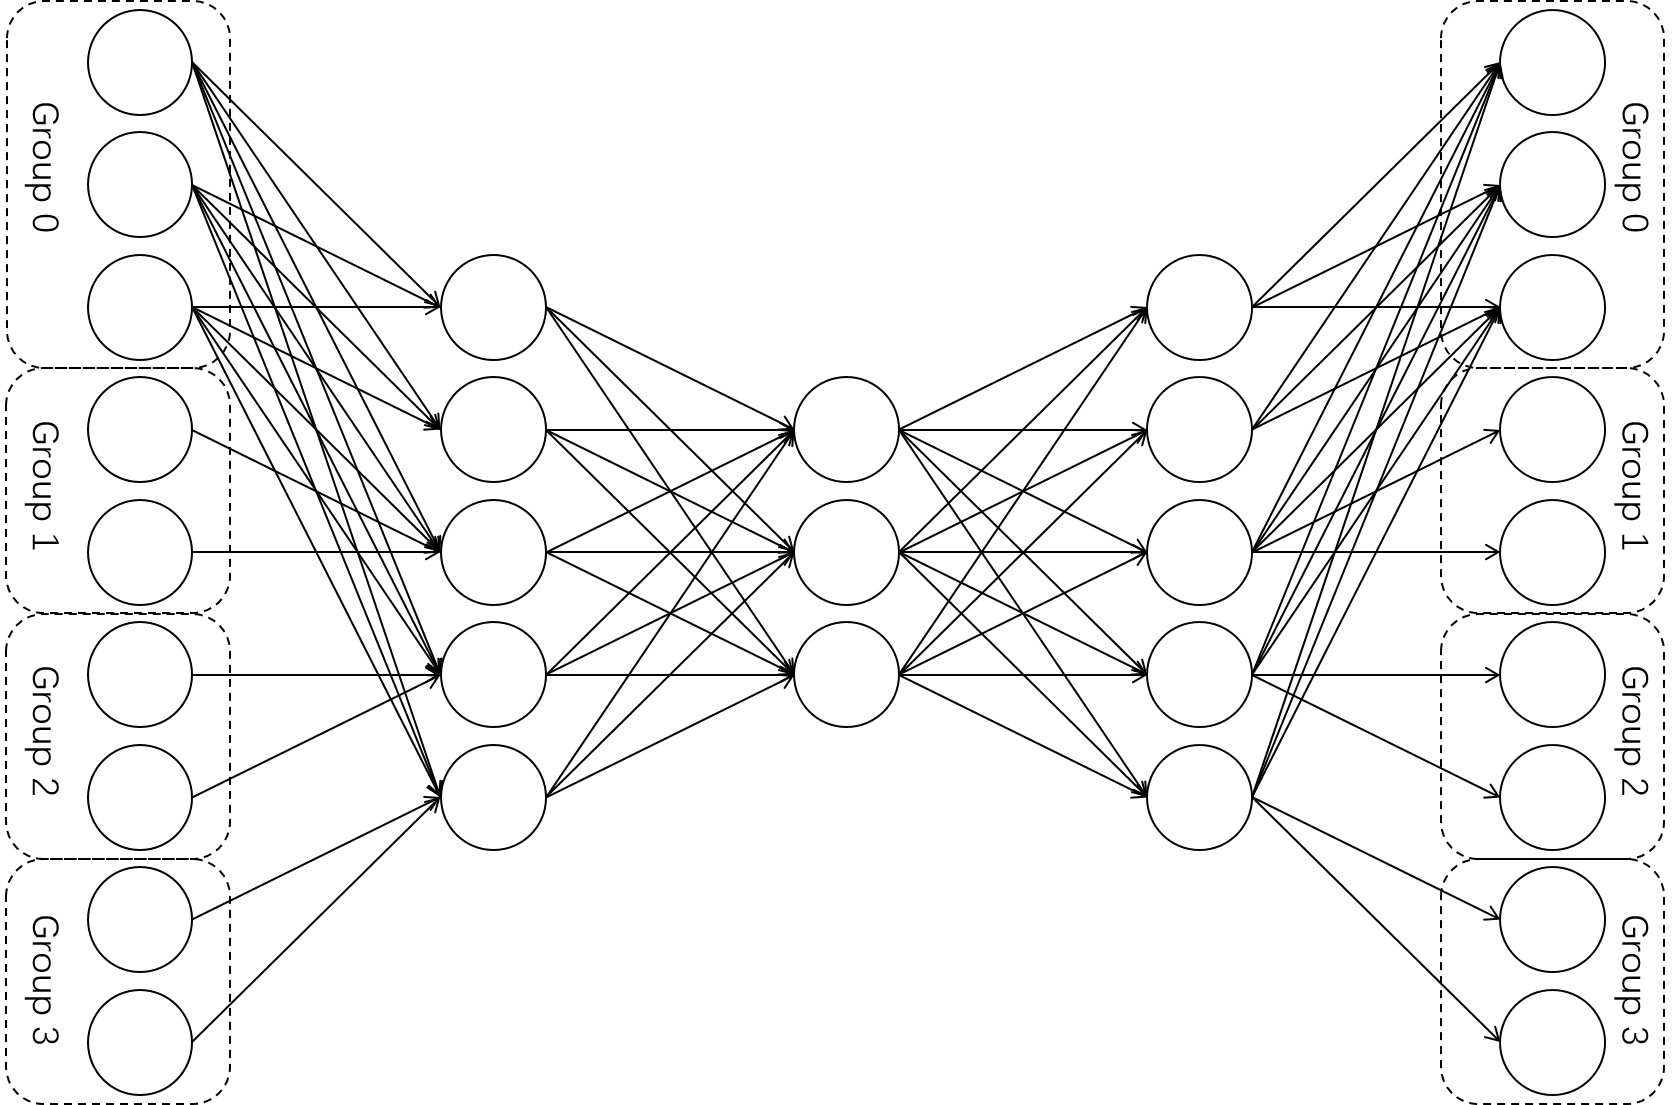
\includegraphics[width=\linewidth]{network.png}
		\caption{Our autoencoder}
		\label{pic:model}
	\end{figure}
	\item {\textbf{Describe your Model:} What approach did you take? What design choices did you make, and why? How
		did you represent the data? How can you evaluate your model for goodness of fit? Did you make an effort to
		identify and exclude irrelevant variables? How did you handle missing data?}
	\par{Given the \ref{interpolation}, we eventually chose to use an autoencoder as our model because it can compress and decompress the given inputs and it is not complicated to build.} 
	\begin{itemize}
		\item {Structure}
		\par{Figure \ref{pic:model} shows the structure of our model.}
		\begin{enumerate}
			\item {The input}
			\par{There are 223 nodes in the input. We scaled the input to be in $ [0, 1] $. Each node could be either in a classification group or in a real value group. The activation function here is ReLU in order to make it less computationally expensive. The dropout rate of this layer is 10\%.}
			\item {Hidden layer 1}
			\par{There are 180 nodes in this layer. The activation function here is ReLU.}
			\item {Hidden layer 2}
			\par{There are 100 nodes in this layer. The activation function here is ReLU.}
			\item {Hidden layer 3}
			\par{There are 180 nodes in this layer. The activation function here is ReLU.}
			\item {The output}
			\par{There are 223 node in the output.  The activation function here is Sigmoid in order to make values lie in $ [0, 1] $.}
		\end{enumerate}
		
		\item {Loss/Error}
		\par{We are measuring the reconstruction errors. For the reason that there are many data types, we are treating the data over different loss functions.}
		\par{For real values and integer values, we are using mean squared error (m denotes the number of data points) \[ L_{MSE}(\theta) = \frac{1}{m}\sum_{i=1}^{m}(\underline{y}^i - \underline{p}^i)^2 , \]   and root-mean-squared error \[ L_{RMSE}(\theta) = \sqrt{L_{MSE}(\theta)}. \]}
		\par{For categorical values, we first converted them to one-hot encoding, then we are treating the problem as a multi-label classification problem (for these categorical values only). Thus, for categorical values, we are using binary cross-entropy loss \[ L_{BCE}(\theta) = \frac{1}{m}\sum_{i=1}^{m}[\underline{y}^i \log (\underline{p}^i) + (1 - \underline{y}^i) \log (1 - \underline{p}^i)]). \]}
		\par{Because the data set is a combination of different types of data, we are using a combination of different loss functions.}
		
		\item {Data}
		\par{This is included in \ref{preprocessing}. We are only training over part of the features. For real values data, we scale it into $ [0, 1] $. For categorical data, we used one-hot encoding to represent which also make the data lie in $ [0, 1] $. Basically all data are in $ [0, 1] $ and we treated all of them as float numbers. }
		\par{We manually removed some irrelevant features such as participant ID. We don't think we are able to train over these features.}
		\par{When dealing with missing features, we have a mask to let us know which feature is missed and then we don't need to calculate loss on this feature.}
	
		\item {Other facts}
		\par{Since we already grouped features as Figure \ref{pic:model} shows, we can first encode each groups and then encode the whole data points. In this way, we can dramatically eliminate the number of weights because our first layer is not dense.}
		\par{Notice that we encode the multiple choice columns into several features. Therefore, we can append a softmax layer to each multiple choice column. One thing to notice that for non-choice features, we have to directly output its value instead of pass it to softmax layer, or it will always return 1. (When we are writing this report, we notice that we can expend each non-choice features into 2 features $x$ and $\bar x = 1-x$. In this case, we can directly pass all features of the same column to a softmax, instead of using masks to identify non-choice features.)}
		\par{Here is another interesting but not necessarily useful fact. Notice that we assumed the rank of this matrix is limited. Namely the transformation can actually be linear. Namely we literally can multiply 2 small matrices to get this matrix. Therefore, we can further define this problem as find 2 matrices $A$ and $B$ to minimize $||M - AB||$, which is literally an optimization problem. But the drawback is that we ignore the meaning of each feature, say sum of several features should always be $1$. But it might be not a bad start, and we can further use Ada boost to combine it with our AutoEncoder.}
	\end{itemize}
	
	\item {\textbf{Describe your Training Algorithm:}}
	\par{We implemented a gradient-based optimizer--stochastic gradient descent with back-propagation for the training part. Comparing with other types of gradient descent, stochastic gradient descent uses one data point at a time, which is computationally friendly. We are only training over 223 features. Our training process was actually quite fast, so we didn't do any compromises.}
	
	\item {\textbf{Describe your Model Validation:}}
	\par{Though there are only about 2400 data points, and it is relatively too small in terms of sample complexity, we can still apply cross-validation. The main idea is here: our goal is predicting blanks given an incomplete data points, and we do have much more incomplete data points if we further randomly set some features to blank. In this way, we can inflate the size of our dataset. Therefore, we randomly divide these 2400 points into train, dev and test set with the ratio 8:1:1. Then we apply dropout method to inflate the train set to meet the requirement of sample complexity. Note that we will not inflate dev and test set because training set is the only set related to building our model. Notice that another advantage of dropout is: Because we are dealing with missing data and trying to interpolate missing data, drop-out makes the model be used to incomplete input data.
}
	\par{During the training process, we measure loss on train set and dev set. Dev set is an indicator of fitness and has been used in fine-tuning of the hyperparameters. If dev loss starts to climb up, we could know it is overfitting. After we finish the training of the model, we evaluate loss on test set.
}
	\par{After the training, our model achieved a low loss of 20.525512.}
	
	\begin{table}[H]
		\centering
		\begin{adjustwidth}{-1.35cm}{0cm}
			\begin{tabular}{|l|l|l|l|l|l|l|l|l|l|l|}
				\hline
				\multicolumn{11}{|c|}{Real-value features our model is good at predicting}  \\ \hline
				Avg. Loss     &      0.00092 &  0.00290 &   0.00776 &   0.01832 &  0.02193 &  0.02628 & 0.02976 &  0.03920 &   0.04213 &   0.04819    \\ \hline
				Column           &     69  & 66  & 102 & 117 & 21  & 22  & 4   & 95  & 255 & 116    \\ \hline
				\multicolumn{11}{|c|}{Probability features our model is good at predicting} \\ \hline
				Avg. Loss     &     0.00003 & 0.00007 &   0.00989 &   0.01377 &  0.01505 &   0.01529 &  0.01724 &   0.01738 &  0.01812 &   0.02385    \\ \hline
				Column           &     7   & 8   & 128 & 101 & 68  & 115 & 94  & 127 & 14  & 170   \\ \hline
				\multicolumn{11}{|c|}{Real-value features our model is bad at predicting}   \\ \hline
				Avg. Loss     &     0.27996 & 0.24402 & 0.23568 & 0.22732 & 0.22094 & 0.21548 & 0.21410 & 0.20914 & 0.20474 & 0.20456   \\ \hline
				Column           &     103 & 63  & 58  & 61  & 111 & 27  & 60  & 90  & 62  & 55     \\ \hline
				\multicolumn{11}{|c|}{Probability features our model is bad at predicting}  \\ \hline
				Avg. Loss     &     0.63081 & 0.24859 & 0.23935 & 0.23137 & 0.16039 & 0.15684 & 0.15087 & 0.14045 & 0.14010 & 0.13857    \\ \hline
				Column           &     171 & 5   & 36  & 85  & 82  & 269 & 83  & 76  & 78  & 81     \\ \hline
			\end{tabular}
			\caption{Model performance}
			\label{table1}
		\end{adjustwidth}
	\end{table}
	
	\item {\textbf{Evaluate your Model:}}
	
	\begin{itemize}
		\item {Where is your model particularly successful, where does it lack?}
		\par{Generally, our model predicts probability values well, and we can find that most multiple choice responses correspond to the original data point (if any). However, some real value differs much. It is partially because of our linear scaling. Another justification for this is generally continuous regression is harder than multiple classification because of the diversity of possible values. If we have more time, we may consider to further encode some real values into multiple choices by grouping possible values.
}
		
		\begin{figure}[H]
			\centering
			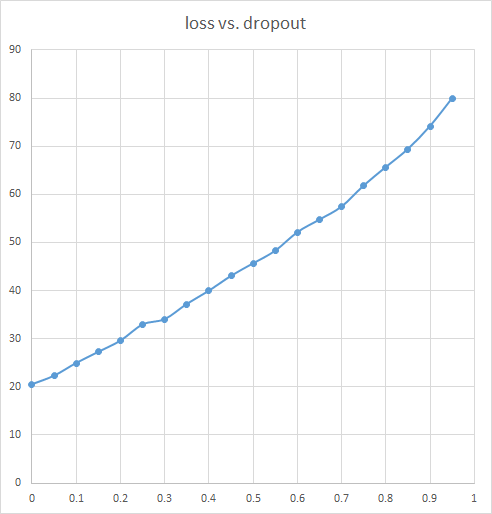
\includegraphics[width=.5\linewidth]{dropout.png}
			\caption{Loss versus dropout rate}
			\label{fig:dropout}
		\end{figure}
		\item {Does it need a certain amount of features in order to interpolate well?}
		\par{In order to answer this question, we apply dropout method when predicting data points in test set. Generally, as dropout rate goes up, less and less features remain, and we can focus on the relationship between prediction loss and dropout rate. The result is shown in Figure \ref{fig:dropout}. 
			
			Notice that when dropout rate is less than 0.4, the curve is basically linear. Namely if there are more than 60\% features are not blanks, we can predict them not bad. Once the dropout rate is higher than 0.4, the loss increases faster. Namely, we cannot predict them properly. A possible justification for this scenario is that when dropout rate is larger than 0.4, many features in group 0 is missed, and it is much harder to predict features crossing different test instead of based on “personality” information (group 0).
		}
		
		
		\item {Are there some features it is really good at predicting and some it is really poor at predicting? Why do you think that is?}
		\par{In order to answer this question, we traced the loss of each feature to the original data, and the result is shown in Table \ref{table1}: }
		\par{Notice that the best real-value feature we predict is L ratio (column 69), and it is really diverse. A plausible explanation is that this effect is ``strong'' enough, and it is true according to the original study (ML3). Actually, the best 3 features (L, K, R ratio) all belong to this effect.}
		\par{The worst real-value feature is sarcasm (column 103). Notice that this effect includes a number of natural language response which we preprocessed roughly, and this effect is also not that significant. Therefore, it is reasonable we cannot predict this feature well.}
		\par{Column 7 and 8 are anagrams 3 and 4, which we encode any word into ``correct answer''. Therefore, it should be the best 2 features because it can literally always predict ``correct answer''. Except these 2 feature, the best probability feature is clipboard weight (column 128), it is interesting because there is no directly related feature except the participant answers. (Note that the clipboard material is independent to its weight.) Namely, we do find that the weight of clipboard will influence participant’s response.}
		\par{The worst probability feature is persistence. (It is a bug actually because I preprocessed it into a probability feature but it actually is a real value. It is my fault. But a good story is it shows we should not use cross entropy to measure the loss of a real-value feature.) The worst feature except for that bugged one is anagrams 1 (column 5). A plausible explanation is that this feature is sort of coincident because we may either happen to have the ``Eureka'' time instantly or be puzzled for a long time and quit this question.}
	\end{itemize}
	
	
	\begin{table}[H]
		\centering
		\begin{adjustwidth}{-1.8cm}{0cm}
			\begin{tabular}{|l|l|l|l|l|l|l|l|l|l|l|}
				\hline
				\multicolumn{11}{|c|}{Most valuable real-value features}   \\ \hline
				Loss diff.    &    0.04869 &  0.04125 &  0.02439 &  0.01700 &  0.01400 &  0.01388 &  0.00923 & -0.00087 & -0.00190 & -0.00317   \\ \hline
				Column             &   255 & 72  & 249 & 248 & 245 & 29  & 253 & 69  & 66  & 246   \\ \hline
				\multicolumn{11}{|c|}{Most valuable probability features}  \\ \hline
				Loss diff.    &   0.29560 & 0.27611 & 0.23960 & 0.23905 & 0.23539 & 0.23360 & 0.22759 & 0.16655 & 0.16586 & 0.09897   \\ \hline
				Column             &   94  & 127 & 115 & 101 & 68  & 65  & 128 & 170 & 36  & 131  \\ \hline
				\multicolumn{11}{|c|}{Least valuable real-value features}  \\ \hline
				Loss diff.    &   -0.29604 & -0.28113 & -0.27959 & -0.25495 & -0.22280 & -0.20728 & -0.20524 & -0.20345 & -0.20235 & -0.19229   \\ \hline
				Column             &   61  & 54  & 104 & 111 & 38  & 27  & 88  & 92  & 252 & 73    \\ \hline
				\multicolumn{11}{|c|}{Least valuable probability features} \\ \hline
				Loss diff.    &   -0.59560 & -0.33963 & -0.22017 & -0.20269 & -0.19237 & -0.19064 & -0.18626 & -0.16885 & -0.16259 & -0.14025   \\ \hline
				Column             &   171 & 85  & 81  & 17  & 19  & 6   & 18  & 84  & 5   & 83    \\ \hline
			\end{tabular}
			\caption{Model performance}
			\label{table2}
		\end{adjustwidth}
	\end{table}

	\item {\textbf{Analyze the Data:}}
	\begin{itemize}
		\item {What features were particularly valuable in predicting/interpolating? What features weren’t particularly useful at all?}
		\par{In order to answer this question, we dropout each feature and calculating the loss after we dropout it. In case of the situation that this feature itself is hard to predict, when we calculating the loss, we will also ignore this feature. The result is in Table \ref{table2}. )
			
			Notice that most of the most important real-value features are aggregated features like NFC, Mood and Agreeableness. It is reasonable because they tell us a whole aspect of this participant, and the response of this participant can be consider as a function of all aspects. (Refer to our transfer learning thought.) Similarly, we can find that most of the least important real-value features are the actual response of each aggregated feature, like intrinsic\_01, selfesteem\_01 and soon. Since they have been aggregated into another features, they do tell us less.
			
			Notice that order of tasks (column 127) does important. It corresponds to the original study design. Some other important features are N position and V position. It is also reasonable because it will determine whether the next response will be greater than 10 or less than 10.
			
			Again, because of my fault, persistence (column 171) become the least important feature. Except for this, the back count features are generally less important. A justification is most participant will correctly answer this question.}
		
		\begin{table}[H]
			\centering
			\begin{adjustwidth}{-1.35cm}{0cm}
				\begin{tabular}{|l|l|l|l|l|l|l|l|l|l|l|}
					\hline
					\multicolumn{11}{|c|}{Real-value features that were changed the least}  \\ \hline
					Difference     &      0.00000 & 0.00000 & 0.00000 & 0.00000 & 0.00000 & 0.00000 & 0.00000 & 0.00000 & 0.00001 & 0.00001    \\ \hline
					Column           &     110	 & 126	 & 109	 & 111	 & 112	 & 113	 & 114	 & 133	 & 75	 & 25	    \\ \hline
					\multicolumn{11}{|c|}{Probability that were changed the least} \\ \hline
					Avg. Loss     &     0.00031 & 0.00056 & 0.02461 & 0.02494 & 0.02606 & 0.02995 & 0.03090 & 0.03194 & 0.03472 & 0.03597    \\ \hline
					Column           &     7	 & 8	 & 20 & 13 & 80 & 18 & 14 & 19 & 11 & 44   \\ \hline
					\multicolumn{11}{|c|}{Real-value that were changed the most}   \\ \hline
					Avg. Loss     &     0.01592 & 0.01004 & 0.00845 & 0.00759 & 0.00745 & 0.00727 & 0.00712 & 0.00653 & 0.00637 & 0.00629   \\ \hline
					Column           &     103	 & 61	 & 54	 & 31	 & 244	 & 60	 & 26	 & 58	 & 35	 & 92	     \\ \hline
					\multicolumn{11}{|c|}{Probability features that were changed the most}  \\ \hline
					Avg. Loss     &     0.63791 & 0.29699 & 0.27964 & 0.26404 & 0.23084 & 0.16518 & 0.14973 & 0.14875 & 0.14656 & 0.14486    \\ \hline
					Column           &     171	 & 36	 & 5	 & 269	 & 268	 & 81	 & 76	 & 82	 & 77	 & 78	     \\ \hline
				\end{tabular}
				\caption{How features change after setting the temperature}
				\label{table3}
			\end{adjustwidth}
		\end{table}
	
		\item {Were there any features about the researcher/experimental environment that were particularly relevant to predicting answers - and if so, what conclusions can you draw about the replicability of those effects?}
		
		\par{In order to answer this question, we choose temperature in lab (column 126) to be coldest or hottest in the given dataset, and compare the predictions. Notice that there is an effect related to temperature (effect 7), and therefore we will ignore all responds in this group. The result is in Table \ref{table3}.
			
			Notice that many columns does not change much, but there are still some columns changed. Sarcasm is changed most in real values, However, since its loss is also relatively high, we cannot conclude that it matters.}
	\end{itemize}
	
	
	
	\item {\textbf{Generate Data:}}
	\par{There are two approaches:}
	\begin{enumerate}
		\item {}
		\par{We picked a complete datapoint and removed part of it, used this to predict the removed features. Then we compared the predicted features and the original features. If they are similar, then we say it's a successful generation. }
		\par{Our model was quite good at this job.}
		\item {}
		\par{To generate a new data point, first we picked a complete data point, then we removed part of it and use the removed data point to predict the removed part. Then we combined the removed data point and the prediction and repeat this process. At last all data from the original data point was removed. }
		\par{To determine whether it's good, we compare the new data point with the original data point. If they are similar, then we say it's a successful generation.}
		\par{Our model was doing alright at this job.}
	\end{enumerate}
\end{enumerate}


\section{Bonus}
\label{sec:Bonus}
\subsection{Dealing with natural language data}
\par{In the dataset, there are several open response columns. Notice that they serve as different functions in the original dataset. In order to try our best to utilize the dataset, we choose to encode them based on their intention in original study.}

\begin{itemize}
	\item {anagrams}
	\par{the first 2 anagram questions have a correct answer, and the other 2 are impossible missions. These 4 questions are used to measure participant's persistence. More specifically, we recorded the time participants spend on these 4 questions. Notice that it is no use to stay at the question have already perfectly answered. Therefore, whether first 2 answers are correct is important. Namely, we encode these features into a Boolean value to indicate whether the answer is correct.}
	\par{Also, we can use our prediction to tell whether the participant would answer correct or not if this feature was blank.}
	
	\item {attentioncorrect}
	\par{It is a trap question to identify whether the participant read the instructions. Generally the other answers will not include the word "instructions". Therefore, we encode any response including "instruction" or similar word into `True`, and further correct some misclassified response manually.}
	\par{In this way, we can predict whether the user inputs "I read the instructions" (or its variants) or missed this check by predicting `True` or `False`}
	
	\item {K L N R V ratio}
	\par{Generally, the response should be a number. Therefore, we checked whether it is a number using Regular Expression, and further rounded these numbers into a nearest integer for our simplicity. For some non-numerical response, we further encode it into numbers or NA manually}
	\par{Once we have the predicted value, we can scale it back to get the ratio that the participant might answer.}
	
	\item {grade 1}
	\par{This question is strongly related to the time participants answer it. More specifically, what this question actually asked is how long it is since the last term. We can get the "current" time in column 222 to 224. Therefore, for this column, we can just encode it into `(month, year)` tuple, and preprocess it into a non-negative integer later. We use regular expression to identify years and seasons and further encode each season into a month. For some irregular response, we encode them manually.}
	\par{When we predicting this column, we first predict the number of months since the last term, and then use "current" time to minus these months and round it into seasons.
	}
	
	\item {grade 2}
	\par{Responses for this question can be consider as a positive number. But generally, there are 3 possible answer types, grades, grade points and percentages. We first use regular expression to identify the type, and then scale all of them into percentages according to \href{https://www.rapidtables.com/calc/grade/gpa-to-letter-grade-calculator.html}{rapidtables}. For some abnormal replies, we encode it manually.}
	\par{Since this column can literally be considered as positive integers, we can directly apply the method of predicting positive integers.}
	
	\item {age}
	\par{(Actually I am wondering why this is an open response question. But anyway,) we can consider this feature as positive integers. We use regular expression to round all numerical responses to nearest integers. Note that any responses are larger than 100 or less than 10 will be consider as NA's. Some non-numerical responses are encoded manually}
	\par{Also, we can predict it just like predicting other positive integers.}
	
	\item {major}
	\par{Since this si a demographical question, what it concerns most is the education background. Therefore, we classify all majors into 8 groups according to \href{https://www.ets.org/s/gre/pdf/dept_major_field_codes.pdf}{ETS}. Though regular expression does not work well in this case, we can discard the prefix "pre-" and sort all responses. In this case, most typos will be aggregated, and we can easily edit their classification using some text editor like sublime text.}
	\par{Generally, this question can be considered as a multiple choice, and we can predict it like other one-hot coding prediction.}
	
	\item {div3filler}
	\par{Actually it is a question to take a period of time. But it actually reflects the mathematical background of this participant. Therefore, we encode it to `True` if all inputs is divisible by 3. Note that there is a $B$ in the question, therefore participant might consider this question is hexadecimal. But it does not matter because $10 = 16 = 1 \mod 3$. We can directly replace $B$ with $2$ and check the sum of all the individual digits. Some irregular responses are coded manually.}
	
	\item {backcount}
	\par{It is similar to div3filler, and we can directly check whether it is correct or not.
}
	
	\item {highpower \& lowpower}
	\par{They are long texts, for simplicity, we skipped them.
}

	\item {tempest1}
	\par{Generally, its responses are positive integers. But some people may answer this quesion in Celsius. Therefore, any value that is less than 40 will be considered as Celsius degree and transformed to Fahrenheit. Furthermore, any value that is greater than 105 or less than 65 will be consider as NA's because it is unlikely to be that hot or cold in labs. Some irregualr responses are coded manually.}
	\par{We can predict this feature like other positive integers.}
\end{itemize}

\subsection{Bonus 2}

\par{Based on available
	features, what can you predict about a person’s answers to natural language questions (if not the actual answers
	themselves)? How can you assess the quality of these predictions?}
\par{We have a thought on this but we don't get the time to implement it.}
\par{Since we already have an autoencoder, we can make use of the encoder to encode non-natural-language data and get the representations. Then we train a neural network to try to predict next word. The input at each time step contains the representations and a word. This word can be encoded using Byte-Pair Encoding or Word Embeddings. The architecture is shown in Figure \ref{rnn}.}
\par{After we finish the training and are going to predict natural language data, we can put representations and <start> into the model. Then we put the first predicted word into the model again. Repeat this process until we get an <end>. This sequence of words is the prediction.}
\par{The quality of prediction can be measured using cross-entropy loss between the prediction and the original sentence. }

\begin{figure}[H]
	\centering
	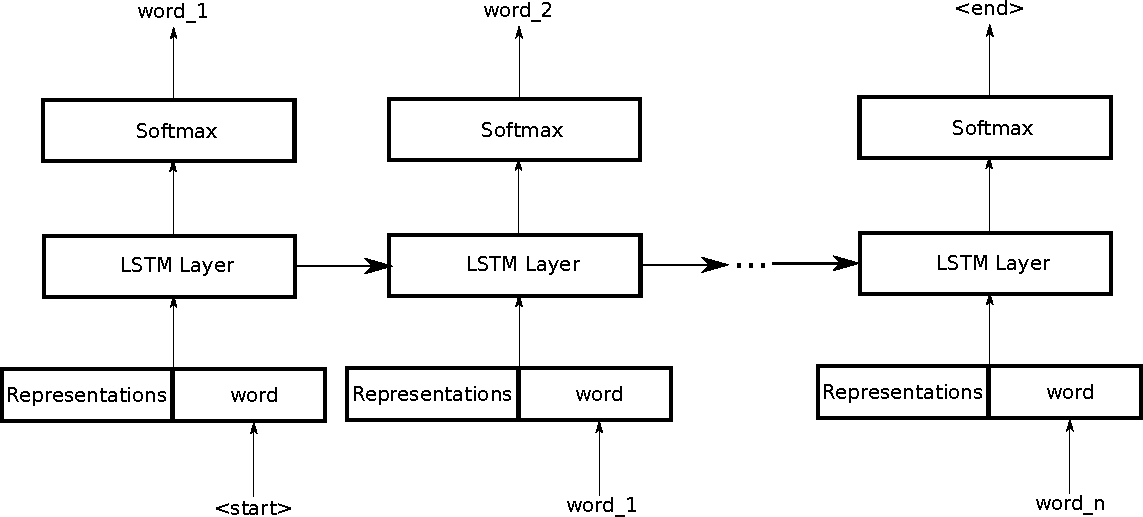
\includegraphics[width=\linewidth]{rnn.pdf}
	\caption{Imaginary architecture of our RNN model}
	\label{rnn}
\end{figure}


\begin{appendices}
	\section{Codebook}
	\label{appendix:codebook}
	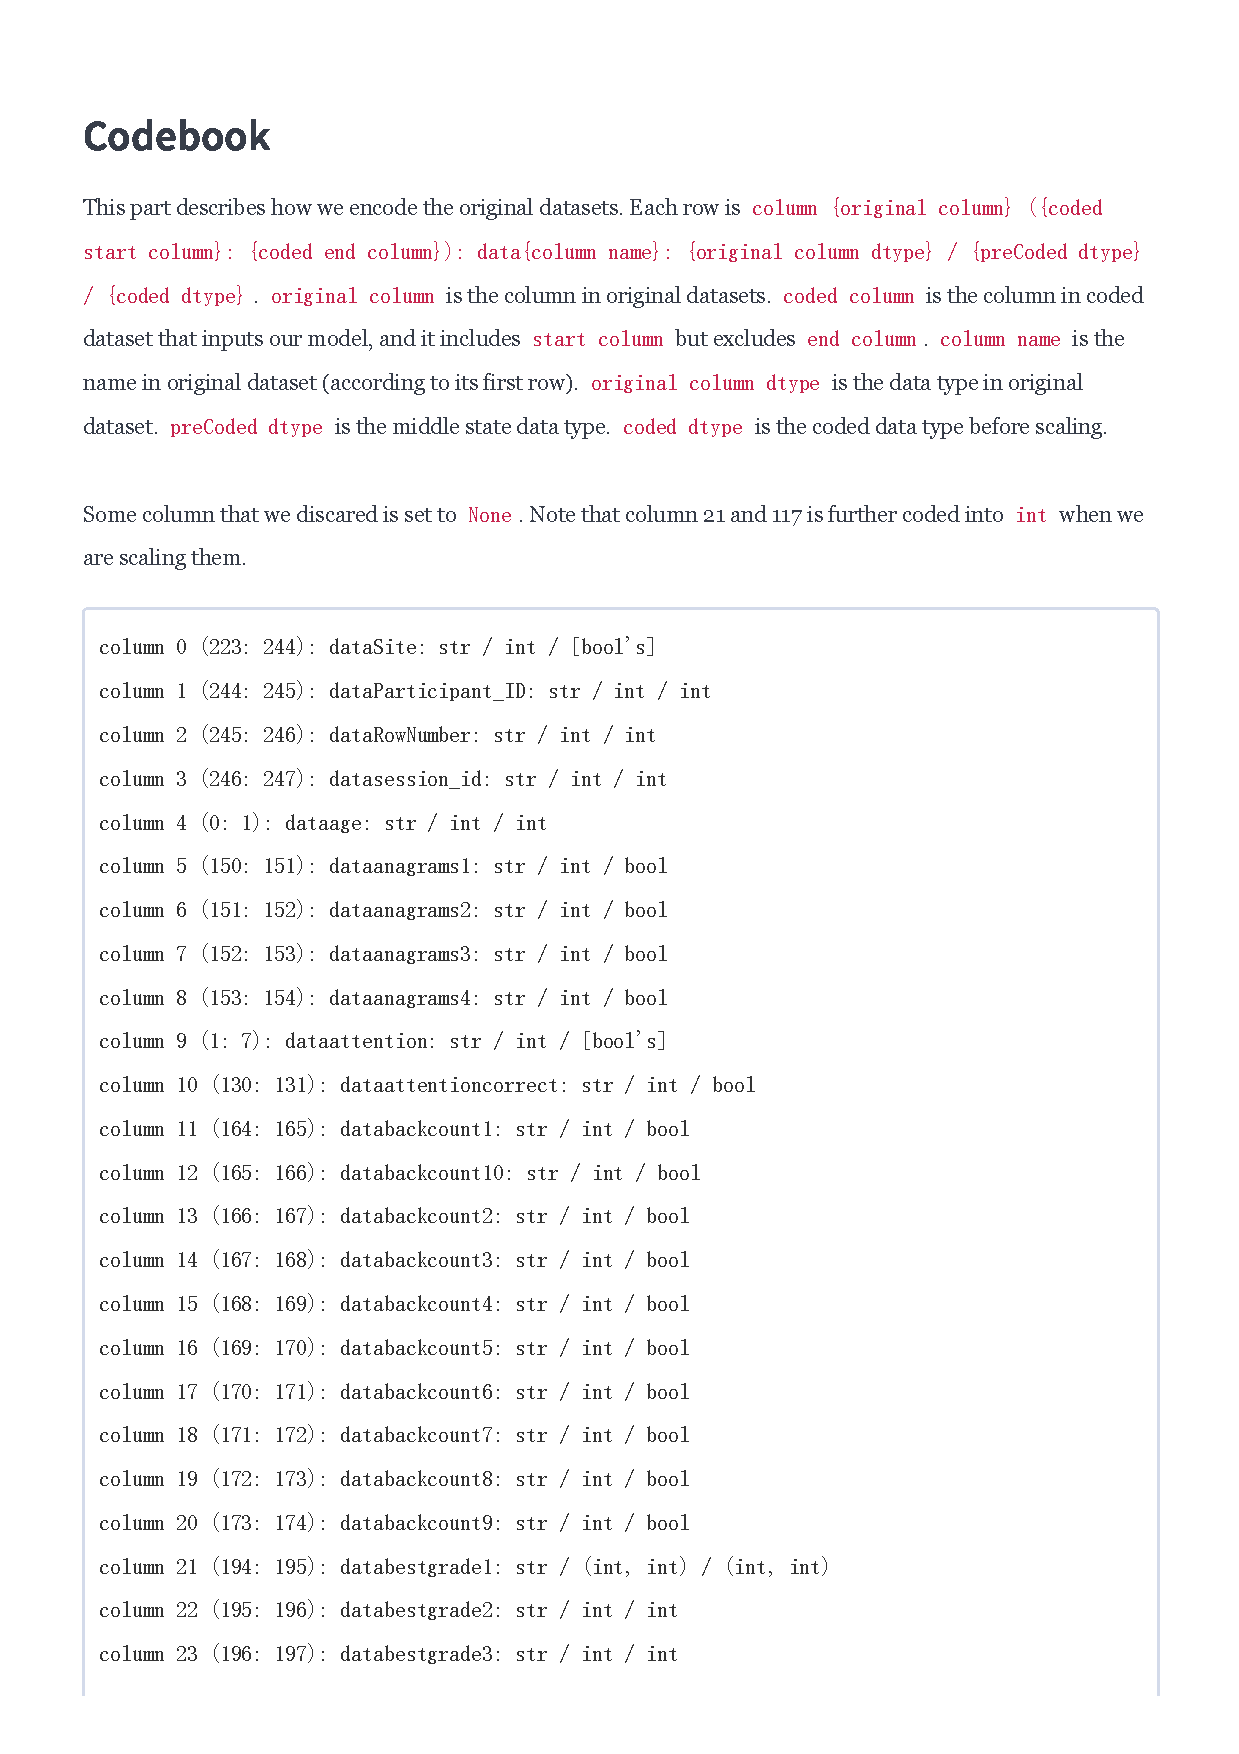
\includepdf[pages=-,pagecommand={},width=\textwidth]{codebook.pdf}
\end{appendices}


\end{document}